% !TEX root=main.tex

\section{Comparison: Relative Edge vs. Pose Optimization}

% show that they are equivalent
It can be plainly observed from comparing Eq~\ref{eqn:global_opt} and Eq~\ref{eqn:relative_opt} that relative edge optimization simply parametertizes the same cost function with relative edge constraints as opposed to global constraints and therefore should result in an equivalent solution.  However, due to the different linearization between the two parameterizations, several simulation studies were performed to show the similarities and differences of global pose and edge-based optimization. Each study focused on the optimization of the pose graph of a house-shaped trajectory, shown in Figure~\ref{fig:house_trajectory}.  This simple trajectory was chosen primarily because the trajectory is simple enough that properly converged graphs are very easy to identify, but also complex enough to illustrate non-trivial items of discussion.  The LevenbergMarquadt optimizer ~\cite{LM Optimization} implemented in GTSAM~\cite{Dellaert2012 - GTSAM} was used as the global pose optimization (GPO) algorithm, while an implementation of Algorithm~\ref{algo:reversed} was used for relative edge optimization (REO).  To evaluate performance of these optimizations, we employed the following RMS error metric, which can be described as the difference between the optimized global pose positions found by optimizer $j$ and optimizer $l$.

\begin{align}
    J_{RMS}(\xhat^j, \xhat^l) = \sum_{i=0}^n \lVert \xhat^j_i - \xhat^l_i \rVert
    \label{eq:RMS_error}
\end{align}

\subsection{Equivalent in Well-Conditioned Case}

The first study illustrates that in a typical, well-conditioned trajectory the optimizations perform equivalently.  The true house trajectory was corrupted with small amounts of random gaussian noise on both translation and heading, had a random selection of edges reversed and a loop closure placed between nodes at the bottom left corner of the trajectory. This was repeated 10,000 times.  Every one of these optimizations produced virtually identical results between global pose and edge-based optimization.  A histogram of RMS error between the global pose of each node of the solution found by both optimizations is shown in Figure~\ref{fig:convergence_house}.  It should be noted that the addition of small translation noise in the trajectory results in a global minima not located at the true trajectory.  This is typical of all pose graph optimizations as described by~\cite{POSE_GRAPH_ERROR}.  Therefore, the optimization approaches are best compared directly with one another, rather than against the ground truth.

\begin{figure}
  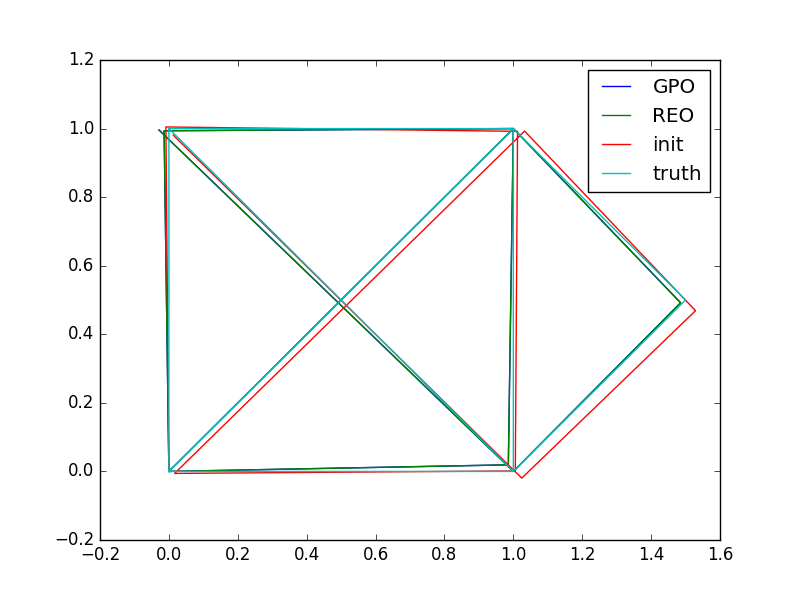
\includegraphics[width=0.7\textwidth]{figures/house_trajectory.png}
  \caption{One sample from the house trajectory simulation study with small errors in both translation and heading with identical optimization results from relative edge optimization and global pose optimization}
  \label{fig:house_trajectory}
\end{figure}

\begin{figure}[H]
  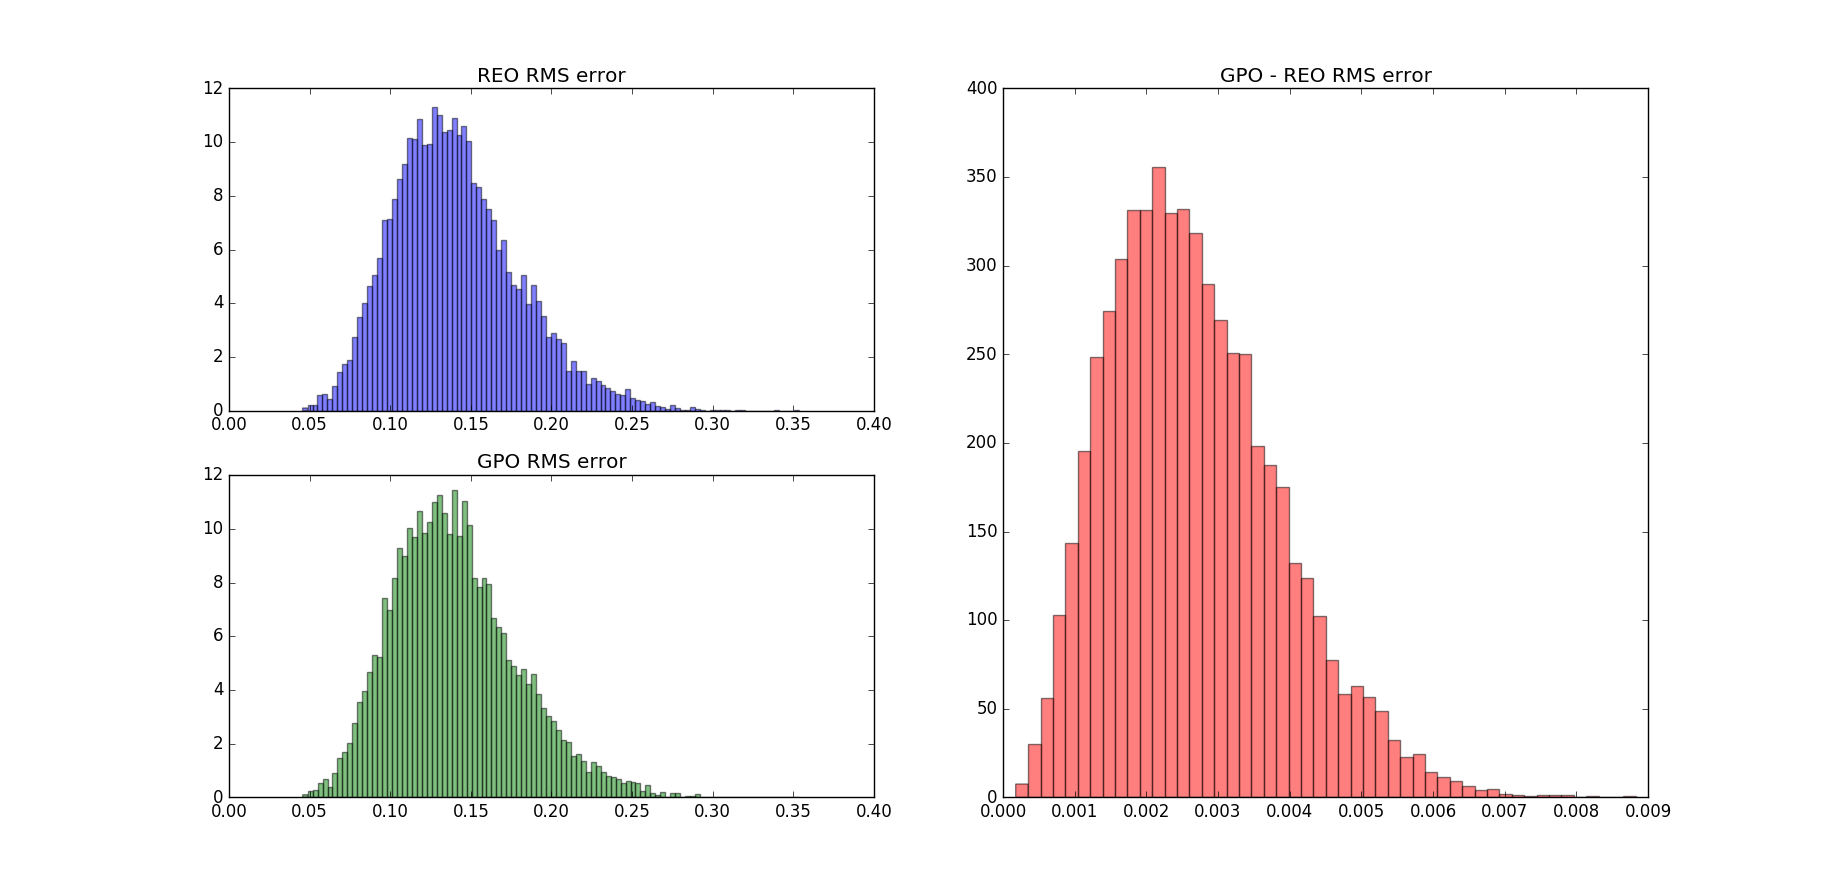
\includegraphics[width=0.7\textwidth]{figures/REO_vs_GPO_good.png}
  \caption{RMS error between optimized poses found by relative edge optimization (REO) and global pose optimization (GPO) for a simulation study of 10,000 house trajectories with small errors in both translation and heading.}
  \label{fig:convergence_house}
\end{figure}

\subsection{Large Heading Errors}
% describe differences (pros/cons)
% Talk about crazy heading error
Differences between the performance of global pose graph and relative edge-based optimizations can be observed by magnifying linearization errors in the underlying parameterization. As a first example, a random house trajectory was generated with perfect translation measurements, but heading errors sampled from $\mathcal{N}(0, 33^\circ)$. Five perfect randomly assigned loop closures were added to the pose graph and the graph was optimized by both GPO and REO.  This process was also repeated 10,000 times.  Figure~\ref{fig:GPO_heading_divergence} shows an example of one of these trajectories, and a histogram of the RMS error of the two approaches is shown in Figure~\ref{fig:GPO_bad_histogram}. REO was able to find the true solution to within 0.001m for 90\% of the graphs, with a max error of 0.0100m and mean of 0.0004585m in an average of 7.546 iterations.  GPO converged to within 0.001m on only a single trajectory, had a max error of 9.825$\times 10 ^{39}m$ and a mean error of 9.856$\times 10 ^{35}$.

\begin{figure}[H]
  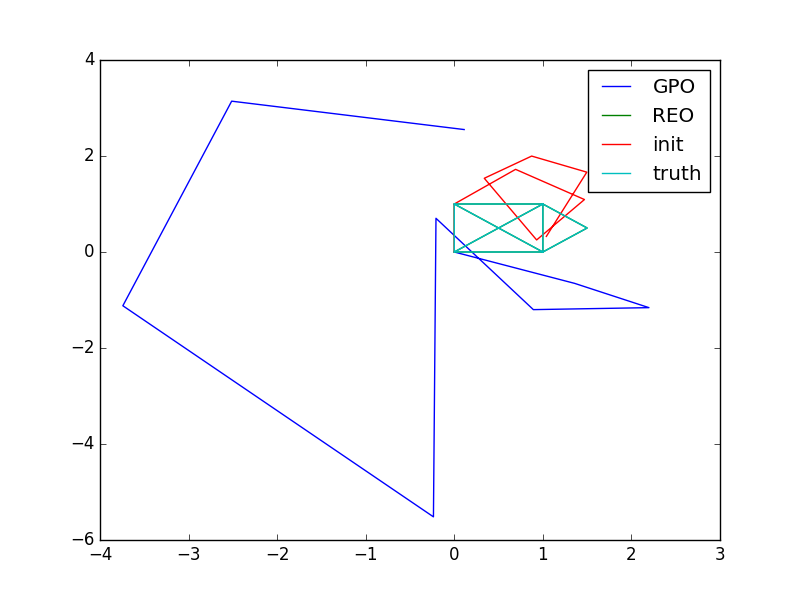
\includegraphics[width=0.5\textwidth]{figures/GPO_diverged.png}
  \caption{One sample from simulation study with perfect translation measurements, five randomly assigned perfect loop closure constraints and significant heading error.  In this case, REO found the true solution while GPO diverged.}
  \label{fig:GPO_heading_divergence}
\end{figure}

\begin{figure}[H]
  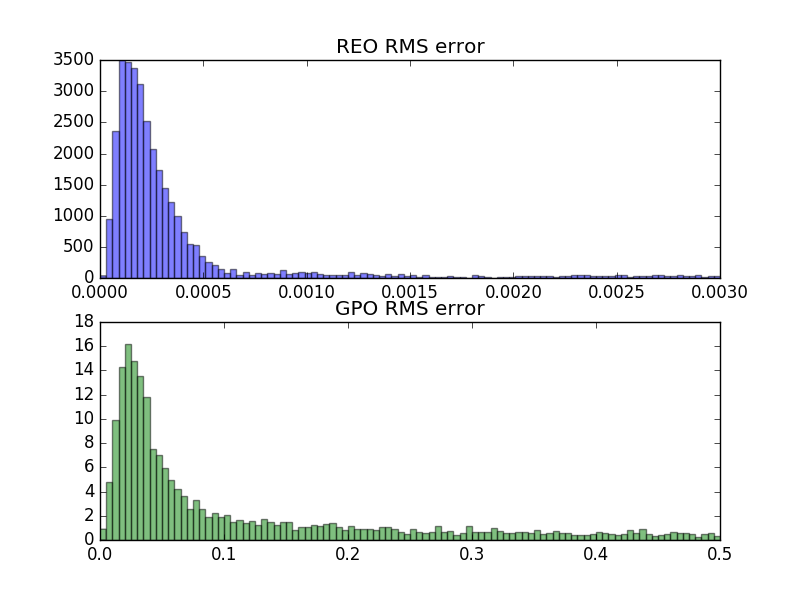
\includegraphics[width=0.5\textwidth]{figures/GPO_vs_REO_bad.png}
  \caption{histogram of RMS error calculated for the final global position of each node after each of 10,000 optimizations with significant heading error, but perfect translation measurements and five randomly assigned, perfect loop closure constraints. The maximum value of RMS error for REO in this study was 0.01004m and the maximum value of RMS error for GPO was 9.825$\times 10 ^{39}m$. Both histograms have been truncated to show details of the histogram at lower values of RMS error despite having quite long tails.}
  \label{fig:GPO_bad_histogram}.
\end{figure}


\subsection{Global Heading Misalignment}

% Talk about bad initialization
A second illustration of the significance in the difference in parameterization can be shown by introducing a large error in initial heading to a pose graph.  This sort of situation often occurs in GPS-denied situations, when, for lack of better information, an agent is initialized in a nominal direction which could be exactly opposite its true global heading.  Only after global measurements are incorporated is the agent able to calculate its original heading.  To illustrate this, we performed a simulation study in which the house trajectory was initialized with varying values of error in global orientation. Small amounts of translation noise ($\mathcal{N}(0, 0.1m)$) and heading noise ($\mathcal{N}(0, 1.8^\circ)$) were applied to each edge and three perfect global measurements were applied using a virtual zero node per the method described in~\cite{CITE}.  In this method, an additional node is placed at the origin of the graph with an infinitely uncertain edge to the first node.  Global measurements are made with respect to this virtual node, therefore allowing the pose graph to shift and or rotate without incurring cost from changing the virtual edge.  Figure~\ref{fig:global_heading_error_trajectory} shows a sample result from this study.

The results of this study, shown in Figure~\ref{fig:global_heading_error_results} illustrate how GPO struggles to optimize this trajectory as initial heading error increase The node at the peak of the house shape is approximately 4 meters away from its initial condition, despite a single edges.  While there are methods which have been shown to handle this issue in pose graph literature, such as~\cite{Paul, others}, when compared with edge optimization, these methods can be described as workarounds to deal with problems inherent in the parameterization.  The fundamental problem is the extremely large position errors which occur in the pose representation due to heading misalignment, and the uneven manifold which the pose representation must traverse in order to arrive at the global minima from a poorly initialized state.  In contrast, edge parameterization typically incurs smaller magnitude errors and therefore easily deals with problems such as arbitrarily large heading misalignment.

\begin{figure}[H]
  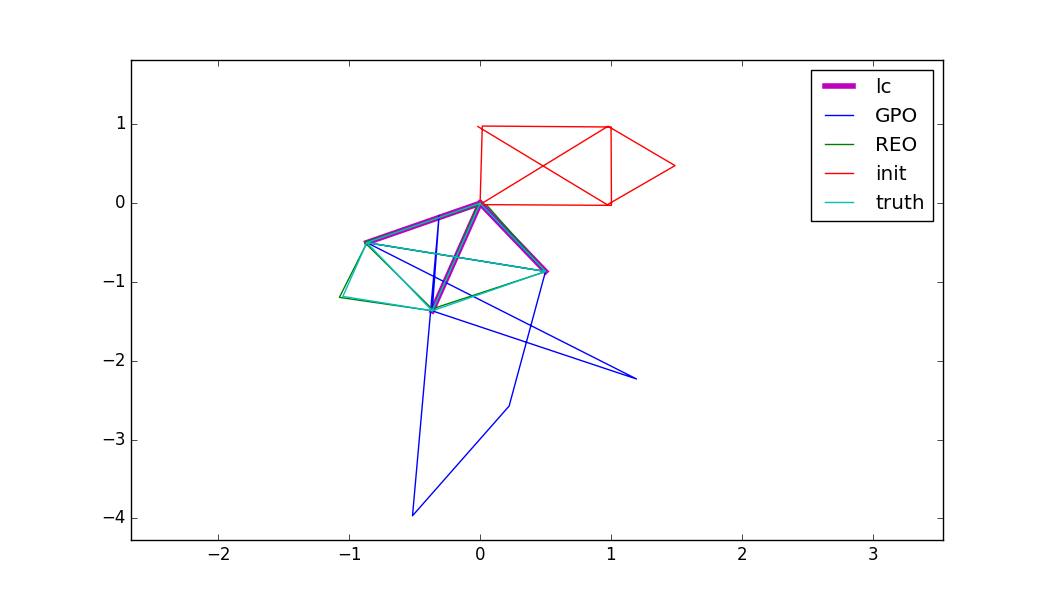
\includegraphics[width=0.7\textwidth]{figures/global_heading_trajectory.png}
  \caption{A sample trajectory where an initial global heading alignment error of $150^\circ$ was applied to a house trajectory.  Small amounts of translation and heading noise were applied to each edge (shown in the init trajectory), and three global measurements were applied (shown in bold magenta) via a virtual zero located at (0,0).  In this case, GPO failed to find the global minima, while REO converged in 7 iterations}
  \label{fig:global_heading_error_trajectory}.
\end{figure}

\begin{figure}[H]
  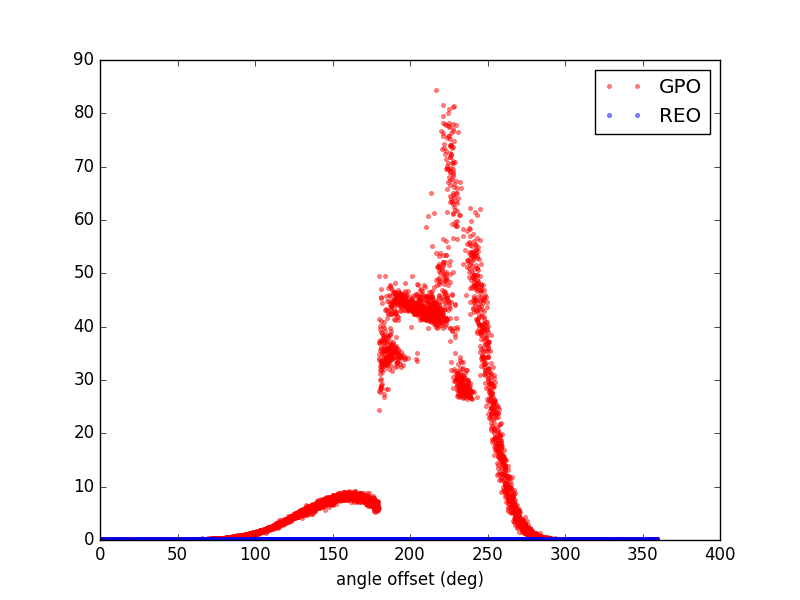
\includegraphics[width=0.7\textwidth]{figures/REO_vs_GPO_global_measurement.png}
  \caption{Results of simulation study where the house trajectory was initialized with different global alignment errors.  Both REO and GPO were supplied with three global measurements, applied using a virtual zero.  As absolute heading alignment error exceeded 60$^\circ$, GPO struggled to find the global minimum.}
  \label{fig:global_heading_error_results}.
\end{figure}

\subsection{Rejection of False Loop Closures}

Another benefit of the relative edge parameterization is the identification of false loop closures.  In REO, if we look at the uncertainty-weighted deviations of each edge in a loop closure, a false loop closure typically has a large number of unlikely deviations in most of the edges which are a part of the loop.   The cost of each loop closure is readily apparent in the evaluation of equation~\ref{eq:edge_update}. To illustrate this, a longer, 'manhattan world' trajectory was generated and provided 10 loop closures.  One of these loop closures was intentionally initialized falsely.  The naive optimization discovered by REO and GPO, without any additional information converged to an incorrect optimum.  If we looked at the deviation of edges in a loop, weighted by the uncertainty on that edge, the weighted RMS error of that particular edge was three orders of magnitude larger than other loops.  The likelihood of such a loop closure being valid is so low, that we can safely remove it from the optimization.  We used a hueristic in which we removed loop closures with a total cost greater than $3\sigma$.  To illustrate this process, a longer 'manhattan world' trajectory was generated and supplied with 10 loop closures, one of which was intentionally false.  GPO and the naive implementation of REO considered this false loop closure and ended up converging to an incorrect solution.  A table of the weighted RMS error on each edge in shown in table~\ref{tab:false_loop_closure}.  Because the false loop closure had a weighted cost greater than $3\sigma$, the robust version of REO correctly identified the false loop closure, rejected it and converged to the proper solution (See Figure~\ref{fig:false_loop_closure})
\begin{table}
  \begin{center}
    \begin{tabular}{|c|c|}
      \hline
      Loop Closure & Cost \\ \hline
      $\mathcal{L}_0$ & 0.001 \\ \hline
      $\mathcal{L}_1$ & 0.001 \\ \hline
      $\mathcal{L}_2$ & 0.001 \\ \hline
      $\mathcal{L}_3$ & 0.001 \\ \hline
      $\mathcal{L}_4$ & 0.001 \\ \hline
      $\mathcal{L}_5$ & 0.001 \\ \hline
      $\mathcal{L}_5$ & 10.00 \\ \hline
      $\mathcal{L}_7$ & 0.001 \\ \hline
      $\mathcal{L}_8$ & 0.001 \\ \hline
      $\mathcal{L}_9$ & 0.001 \\ \hline
    \end{tabular}
  \end{center}
  \caption{ MADE UP DATA Cost of loop closures in manhattan world with a false loop closure while evaluating equation~\ref{eq:edge_update}.  Loop closure $\mathcal{L}_5$ was initialized falsely, and is obiously an unlikely loop closure.}
  \label{tab:false_loop_closure}
\end{table}

\begin{figure}[H]
  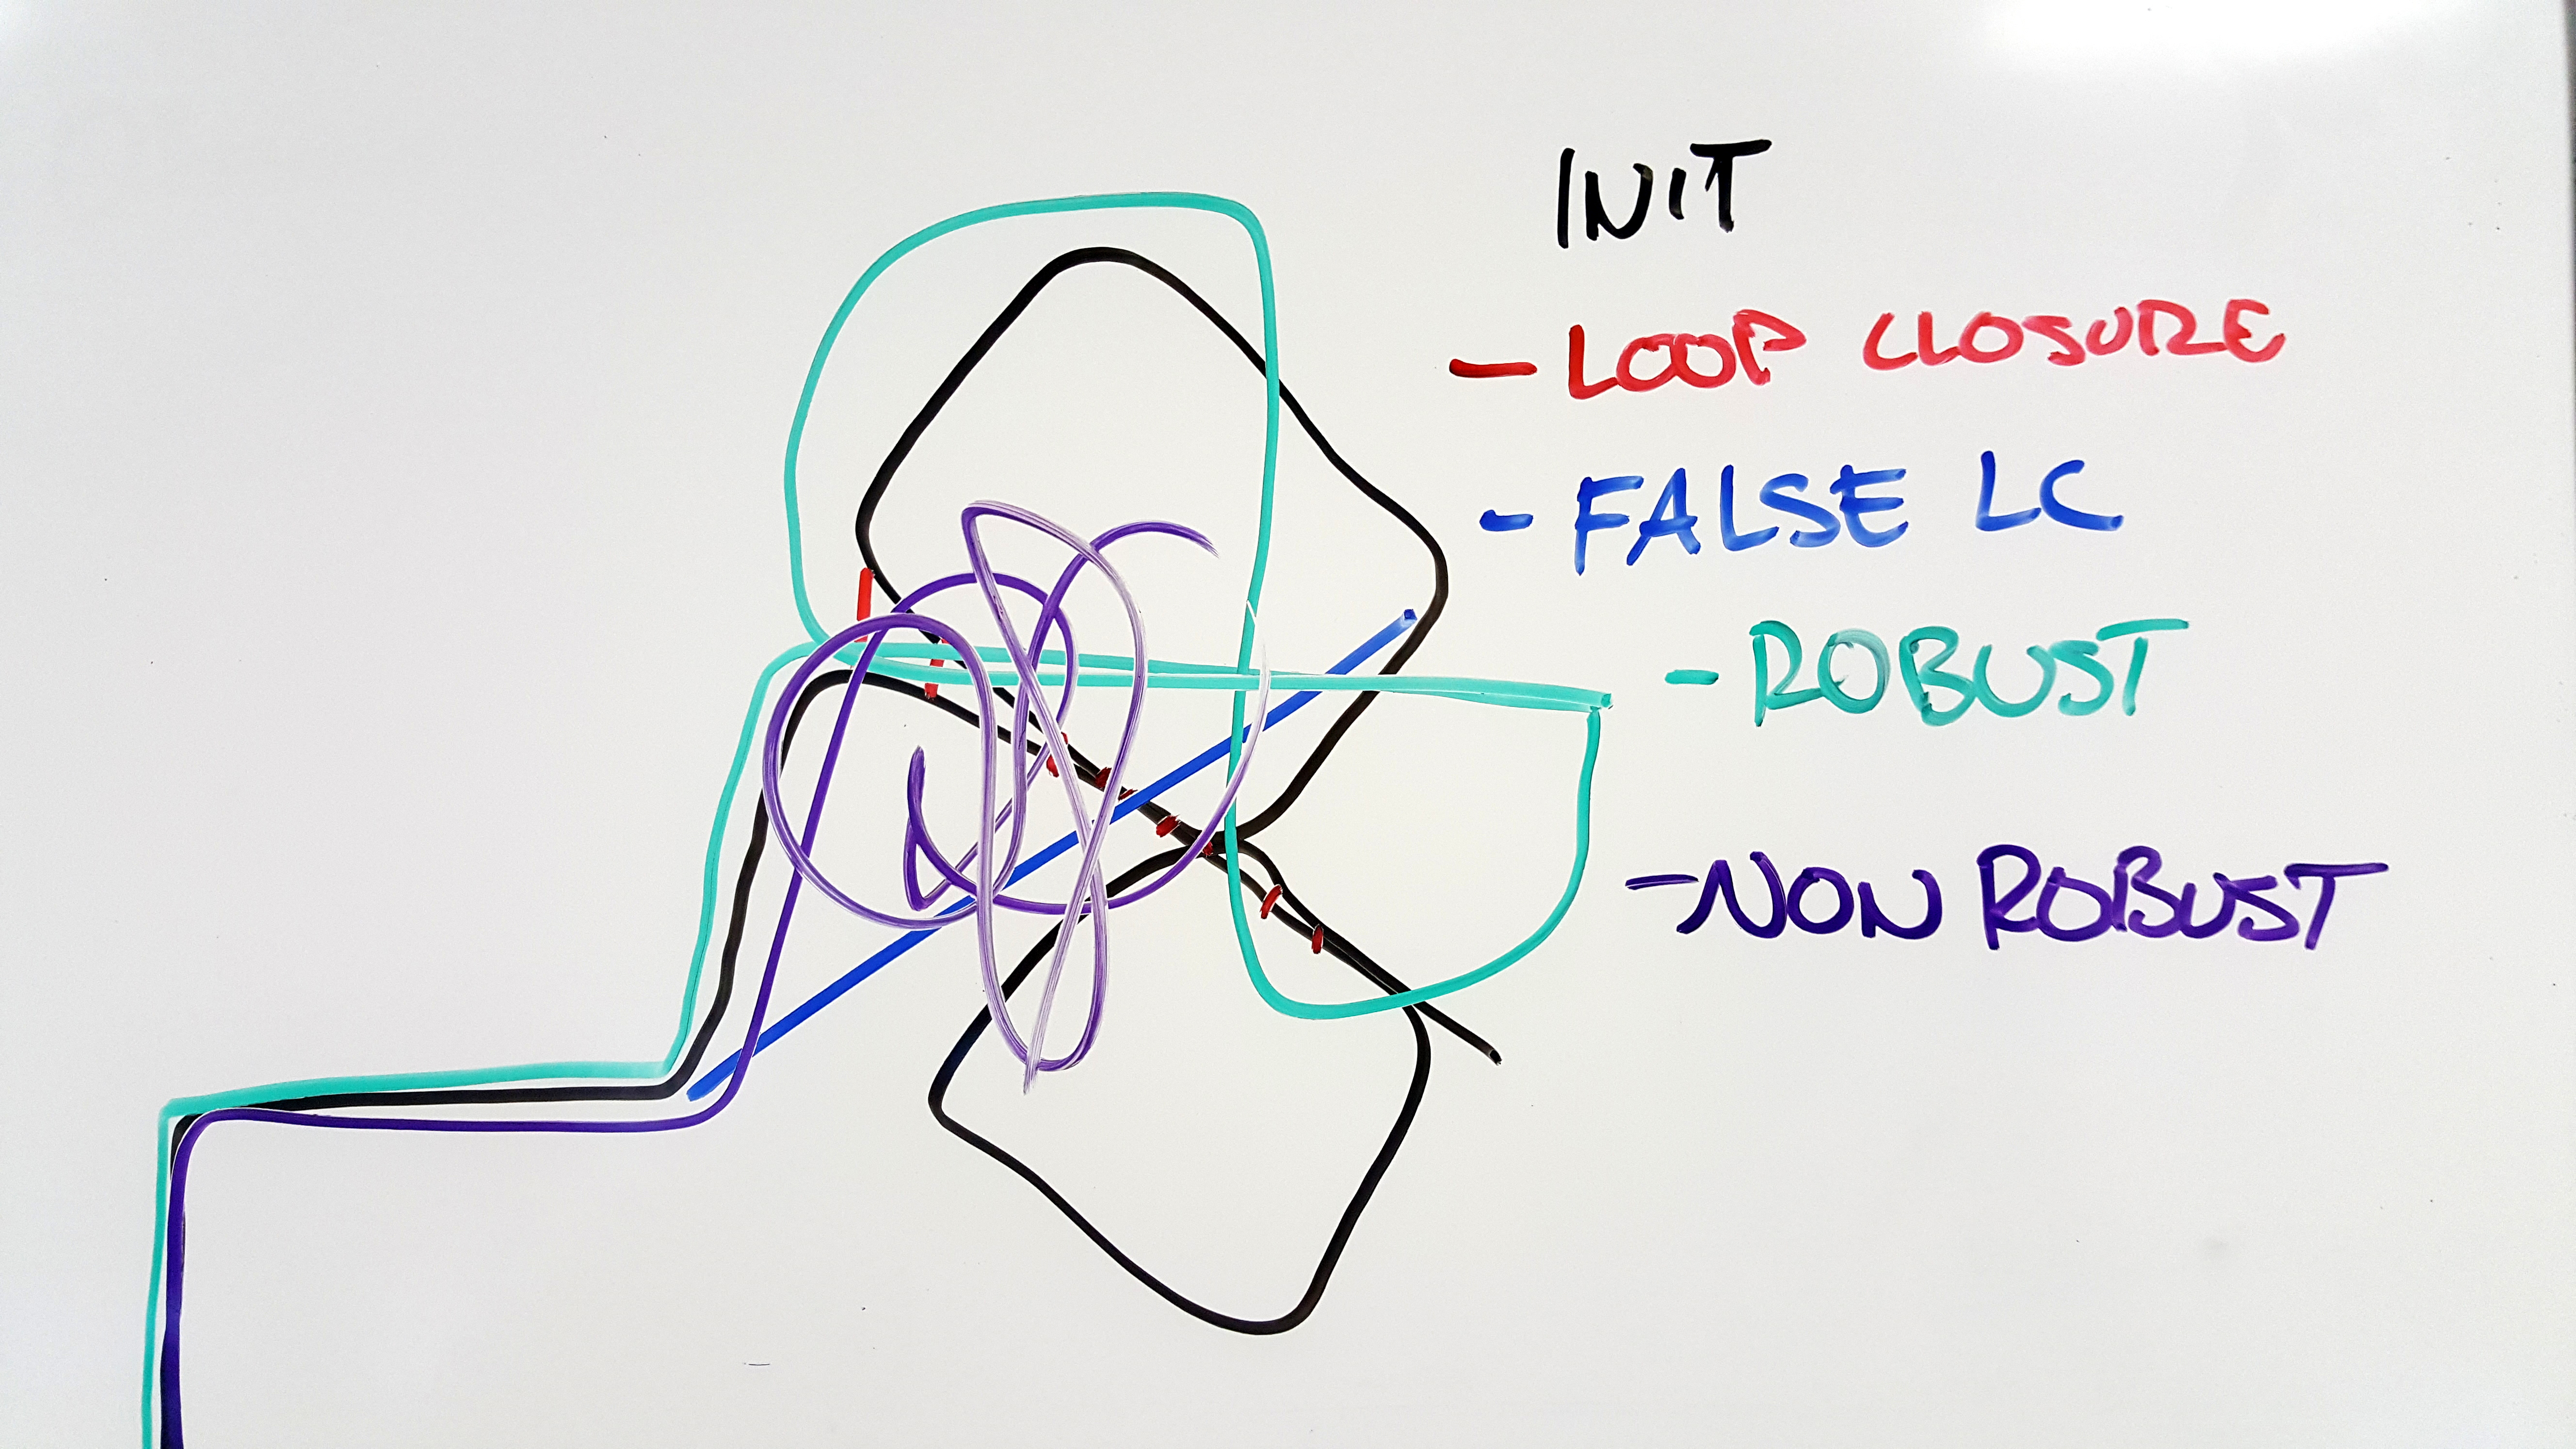
\includegraphics[width=0.7\textwidth]{figures/robust_lc_rejection.jpg}
  \caption{Results of a simulation study with a manhattan world trajectory supplied with 10 loop closures (shown in bold magenta).  One loop closure (shown in red) was falsely applied.  This loop closure was easily identified by the robust version of REO and removed}
  \label{fig:false_loop_closure}
\end{figure}

\subsection{Complementary Nature of Edge and Pose Optimization}

While relative edge optimization promises significant improvements in dealing with initialization errors when compared with global pose optimization, it is not as easily scaleable as global pose graph optimization.  In particular, the calculation of $\frac {\partial\Delta t_{a-z}}{\partial\Delta t_{ij}}$ results in significant correlations between the edges involved in a loop closure.  These correlations ultimately lead to a loss of sparsity in the calculation of $\mathbf{H}_{az}^\top \Omega_{az} \mathbf{H}_{az}$ in Equation~\ref{eqn:3d_opt}.  The parameterization of global pose optimization however, does not run into this issue and can therefore exploit sparsity in solving for $\Delta \mathbf{x}$.  This becomes most important when considering a loop closure with a large number of edges where a dense matrix decomposition can be very costly. Secondly, in typical pose graph implementation, the number of edges can grow explosively if an agent repeatedly navigates the same area.  In this situation, the sum in the second term of the cost function in Equation~\ref{eqn:cost_function} can become extremely large and costly to calculate.

With these shortcomings in mind, we propose that edge optimization be performed for just a few iterations in situations where global pose graphs may struggle to find global minima to initialize the graph.  After a great deal of error has been removed by the more expensive, but more robust edge optimization, global pose graph optimization can very quickly find a global minima even in highly-connected and complicated graphs, where repeated edge optimization may become intractable.

To demonstrate the effectiveness of this strategy, we repeated the global heading error simulation study with a single iteration of REO to initialize the graph, the result of which was then passed to GPO for refining.  In all three situations, the combination of both REO and GPO resulted in strong robustness to initialization errors and resulted in 100\% convergence.

\begin{figure}[H]
  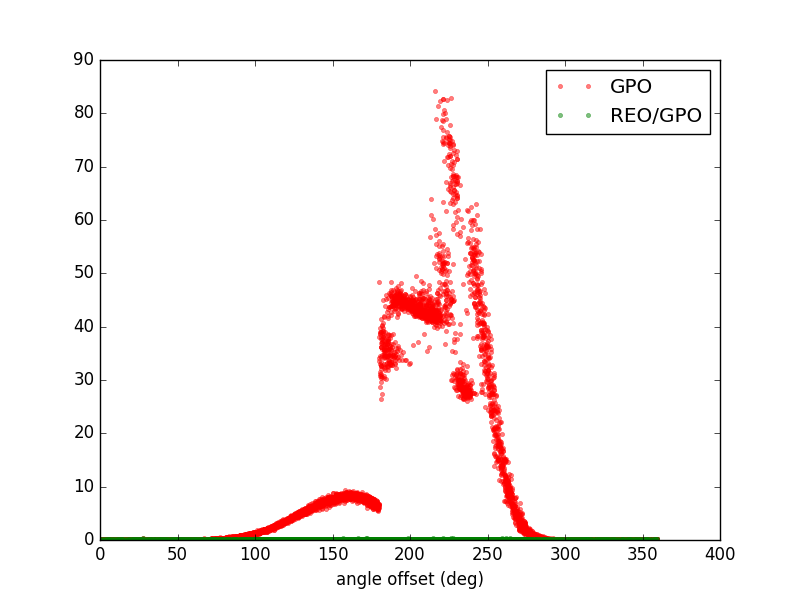
\includegraphics[width=0.5\textwidth]{figures/combined_global_heading_results.png}
  \caption{Results of a second simulation study with varying angles of initial heading error.  In this case, the addition of a single iteration of REO prior to using GPO resulted in perfect convergence, despite large initial heading error.}
  \label{fig:combined_global_heading_results}
\end{figure}

Because we will use GPO to perform the bulk of refining the optimization, and are using REO to primarily remove a great deal of initialization error, we can hueristically choose only a subset of loop closures to optimize.  In highly-connected graphs, it is unlikely that the types of errors which cause GPO to have trouble occur at all.  These issues typically arise in situations of prolonged odometry without loop closures, when merging graphs from several agents, and when first incorporating global measurements into a pose graph.  In addition, because REO struggles computationally when considering a large number of loop closures, we can select and use REO only for these troublesome situations.

To illustrate this point, a large simulation study was performed in a large manhattan world with 100 agents.  These agents were initialized arbitrarily in the world, without knowledge of their global position.  For the sake of plotting and describing the graph, we will discuss the world view of the first agent, initialized in the center of the world.  This is an arbitrary distinction, and any arguments about the first agent could apply to any and all agents. Loop closures were simulated between agents with heading error sampled from $\mathcal{N}(0, 5^\circ)$.  When the first loop closure was detected, the mean translation and rotation consistent with the loop closure was applied to the new pose graph and the graphs were combined.  When a second loop closure was discovered between these agents, 3 iterations of REO was used to align the minimum set of edges describing the loop closure of these new agents with the first.  The mean translation and rotation applied to the edges in this loop were then applied to all edges in the new agent's graph, to align it with the first agent.  After this initial alignment by REO, the two pose graphs were then combined and optimized with GPO.  Any additional loop closures were optimized with GPO directly, under the assumption that the two subgraphs were connected enough to avoid large alignment errors.

This simulation was repeated with increasing error in heading, and a comparison of whether or not the REO initialization step was used to initialize the graph shows that REO is necessary after heading error exceeded $\mathcal{N}(0,5^\circ)$.  The threshold for performing an REO alignment is also likely a function of the time between loop closures, and more robust versions of this alignment algorithm might continue to perform REO alignments after a period of disconnection, because of the compounding of heading error.  This simulation study was performed in real time on a laptop computer, indicating the scalability of using a pose graph optimization as the backend to fuse a map created by multiple agents.

As shown in Figure~\ref{fig:manhattan_world_results}, incorporating agents far away from the origin caused GPO to diverge, primarily because of the compounding heading error which results in a bad initialization for the pose optimization.  Using a relative edge alignment step prior to pose optimization prevented this error from causing divergence.  While an REO-only optimization fell behind real time if used for such complicated graphs, the addition of a 3-iteration REO alignment on a subset of edges prior to global pose optimization incurred a constant 0.001s cost to the optimization but drastically improved robustness.

\begin{figure}[H]
  \includegraphics[width=0.5\textwidth]{figures/manhattan_world_sim.jpg}
  \caption{Results of large simulation study with 100 agents navigating a manhattan world.  Each agent was initialized with no prior understanding of the other agent's locations.  The initial position of the first agent was used as the origin for plotting purposes and for initializing GPO without the REO alignment step.  On the left we see the results of using GPO only.  In this case, the optimization diverged after incorporating agents a long distance from the origin, from the compounding of heading error.  On the right, we see that performing an REO alignment step prevented this from happening and kept GPO robust to this sort of error.}
  \label{fig:manhattan_world_results}
\end{figure}
